\chapter{Variable attenuators}\label{ch:vargain}
	\section{Introduction}

		The IF-signal output should preferably be fixed in power as well as in frequency for later digital to analog-converters to be effective. In order to adjust the signal to a given level, the gain from the amplifiers is slightly higher than needed which, combined with variable attenuators, creates a variable gain circuit.

	
	%	It is specified that the variable gain should be controlled digitally, with \unit[3-4]{bits} of resolution and a gain of \unit[$\pm5$]{dB}, see \autoref{app:specs}. All attenuators are matched to \unit[50]{$\Omega$}. Bandwidth is not considered as the signal, after the mixer, has a narrow frequency band of \unit[20]{MHz} at \unit[2.14]{GHz}.  There are already variable attenuators implemented in PH25 and a comparison between basic attenuators in PPH25 concludes that there is little point in choosing another type.\autocite{gustavsson07}


	\section{Topologies}
		
		The simplest attenuator consists of a resistance that somehow interacts with the main RF line. Usually transistors are used to dynamically divert power into an attenuator, either into ground or back to the main line. This crude technique will however lead to relatively large reflections which is why slightly more sophisticated topologies are used. T- and $\Pi$-attenuators are common and offer small reflections, see Figures \ref{fig:tee_att_simple} and \ref{fig:pi_att_simple}.


		
		A fairly thorough discussion by \citeauthor{gustavsson07} concludes that due to compact size and ease of control, the T-structure makes the best choice of attenuator.\autocite{gustavsson07} The same arguments are valid for this circuit and process and thus the same type of attenuator is implemented. No notable differences are seen between PH25 and PPH25.

		\begin{figure}[ht]
			\begin{minipage}[b]{0.5\linewidth}
				\centering
				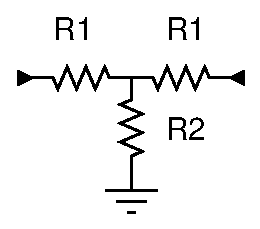
\includegraphics[width=0.5\textwidth]{fig/attenuators/tee-attenuator-symbolic}
				\caption{A tee-attenuator.}\label{fig:tee_att_simple}
			\end{minipage}
			\hspace{0.5cm}
			\begin{minipage}[b]{0.5\linewidth}
				\centering
				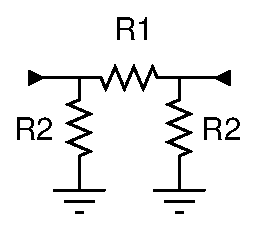
\includegraphics[width=0.5\textwidth]{fig/attenuators/pi-attenuator-symbolic}
			\caption{A pi-attenuator.}\label{fig:pi_att_simple}
			\end{minipage}
		\end{figure}

	\section{Design}

		The values of the resistances $R_1$ and $R_2$ for the T-attenuator are given as \autocite{matthaei80}
		\begin{align*}
			R_1 &= Z_0 \left[\frac{10^{A/20}-1}{10^{A/20}+1}\right] \\
			R_2 &= 2Z_0 \left[\frac{10^{A/20}}{10^{A/10}-1}\right]
		\end{align*}
		In order to control the attenuator, two FET's are added between the tee-pad and ground and in parallel with the tee-pad, see \autoref{fig:tee_att_symbolic}. When V1 is closed and V2 open, there is no attenuation. Opening V1 and closing V2 forces the current to go through the resistances and partly into ground resulting in an attenuation.

		The attenuators are  biased by giving the source \unit[+5]{V} and switching  the gate voltage between \unit[3]{V} and \unit[5]{V}. Therefore a DC-block must be added between V2 and ground in \autoref{fig:tee_att_symbolic}. 
		
		\begin{figure}[h!]
			\centering
			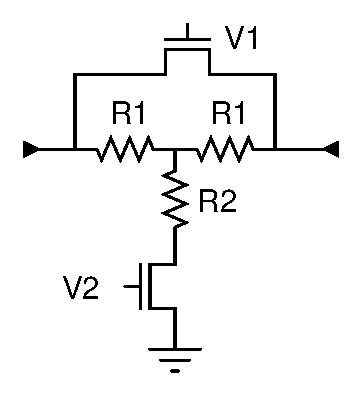
\includegraphics[width=0.4\textwidth]{fig/attenuators/tee-attenuator-variable-symbolic}
			\caption[A tee-attenuator schematically]{A tee-attenuator schematically. By switching the FETs, the gain is changed. When V1 is shorted and V2 open, the attenuator is not active. By reversing the voltages, the attenuator is activated.}\label{fig:tee_att_symbolic}
		\end{figure}



		The values of $R_1$ and $R_2$ are optimized to account for the extra capacitor and FET parasitics. The gates of the FETs are connected via high-value resistors to the control blocks. The high-value resistors are added to increase the FET's $S_{21}$ in its closed state, see \autoref{fig:fet_gate_resistance}. A \unit[6]{k$\Omega$} resistance is chosen, as in the PH25-process. 

		

		\begin{figure}[h!]
			\centering
			\includerect{0.7\textwidth}{fig/fet_gate_resistance}
			\caption[Drain-source conductance depending on gate impedance.]{The inherent attenuation of the FET in its closed state, depending on gate impedance for the switching FET  (PPH25SSW).}\label{fig:fet_gate_resistance}
		\end{figure}		
		
		\begin{figure}[h!]
			\centering
			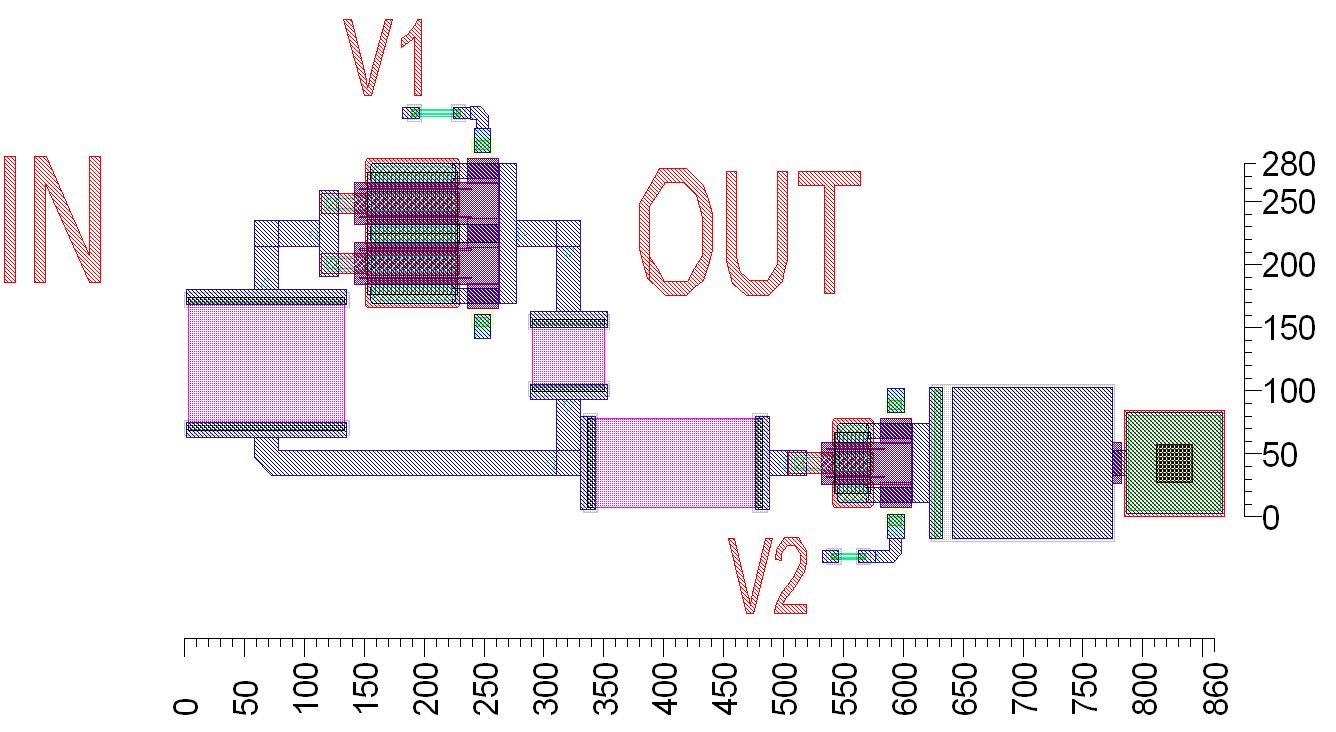
\includegraphics[width=1.0\textwidth]{fig/attenuators/tee_att_layout_6dB}
			\caption[Layout of a tee-attenuator]{Layout of the 6dB-attenuator.  A high-value resistor is connected to the gate of the FETs.\scalemum}\label{fig:tee_att_layout}
		\end{figure}
		
		%6dB att: Max 40mA on $R_0$ and 22mA over $R_1$ when sending 16dBm across. With 0.4mA/\mum, the width has to be 100 and 55 respectively.
		% I0, I0, I1 => W0, W0b, W1
		%6dB: 53, 25, 28mA
		%3dB: 60mA, 43, 18mA => 150, 110, 45
		%1.5dB: 45mA, 40mA, 6mA => 110, 100, 15
		
			

	\section{Combining attenuators}

		Several techniques are available when combining attenuators to achieve a spectrum of discrete points. Attenuators can be connected in parallel or in series. A parallel connection results in a smaller total loss when all attenuators are inactive, i.e. when maximum gain is sought. This is because of the inherent drain-source resistance in the transistors used for overriding the attenuators. When connecting attenuators in parallel, the total loss is smaller in their inactive state but there are fewer possible states of attenuation.

		As maximizing the number of controlling bits and thereby saving chip-size is deemed important, it is decided to use a series design of the attenuators. Furthermore, a resolution of \unit[1.5]{dB} and a total of \unit[3]{bits} suffices. This gives $2^3=8$ steps and a maximum attenuation of $1.5+3+6=\unit[10.5]{dB}$.

%		If the free chip-space allows it in the end, one possibility may be to add an additional \unit[0.8]{dB} attenuator. %TODO at end of project, is this still valid?

The entire attenuator-circuit must be properly biased. Therefore there are DC-blocks before and after the attenuators. The entire line is raised to \unit[+5]{V} by connecting the bias-voltage through a high-resistance element serving as IF-block (\autoref{fig:attenuator-chain-symbolic}).

		\begin{figure}[h!]
			\centering
			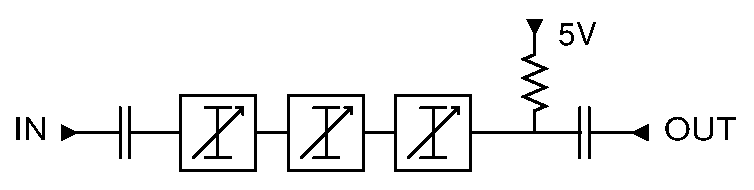
\includegraphics[width=0.8\textwidth]{fig/attenuators/attenuator-chain-symbolic}
			\caption[The attenuator-circuit schematically]{The three attenuators with DC-blocks raised to \unit[5]{V} so that the FETs are properly biased. The attenuators are controlled by level-shifters as explained in the following chapter.}\label{fig:attenuator-chain-symbolic}
		\end{figure}

	
	\section{Results}
		
		When simulating the attenuators, there is the option of using a linear model of the switching FET called PPH25SSW or the non-linear cold FET called PPH25NCF. The non-linear models are more powerful in that they can be used in non-linear simulations but the linear switching FET  models approximate linear operation better. The simulations are performed with PPH25SSW as far as possible.		
		
		The attenuation values and reflection coefficients for all attenuators are displayed in \autoref{tab:VarGainData}. All attenuation states, including spread are seen in \autoref{fig:All_attenuators_spread}. The compression point, $P_{1dB}$, for the complete variable-gain-circuit (three attenuators in series) is calculated to \unit[22]{dB} using PPH25NCF when all attenuators are in their inactive state. All other states result in higher $P_{1dB}$.
	
	
	
		\begin{table}[h!]
			\caption{Simulated attenuator data for PPH25SSW.}
			\label{tab:VarGainData}
			\centering
			\begin{tabular}{ l l l l } \toprule
				Attenuator & 	$S_{21,\text{diff}}$ &	$S_{21,\text{off}}$ &  $S_{11}$, $S_{22}$ \\\midrule
				\unit[1.5]{dB} & \unit[1.5]{dB}	&	\unit[0.36]{dB} & $>$\unit[25]{dB} \\
				\unit[3]{dB} & \unit[3.0]{dB}	&	\unit[0.34]{dB} & $>$\unit[25]{dB} \\
				\unit[6]{dB} & \unit[6.1]{dB}	&	\unit[0.35]{dB} & $>$\unit[21]{dB} \\\bottomrule
			\end{tabular}
		\end{table}


%		\begin{figure}[hbt!]
%			\centering
%			\includerect{1.0\textwidth}{fig/attenuators/S_params_1_5dB}
%			\caption[The S-parameters of the 1.5dB attenuator]{The S-parameters of the 1.5dB attenuator with switching FET. Spread is included as a TiWiSi-resistor is used which has a large spread.}\label{fig:S_params_1_5dB}
%		\end{figure}

%		\begin{figure}[hbt!]
%			\centering
%			\includerect{1.0\textwidth}{fig/attenuators/S_params_3dB}
%			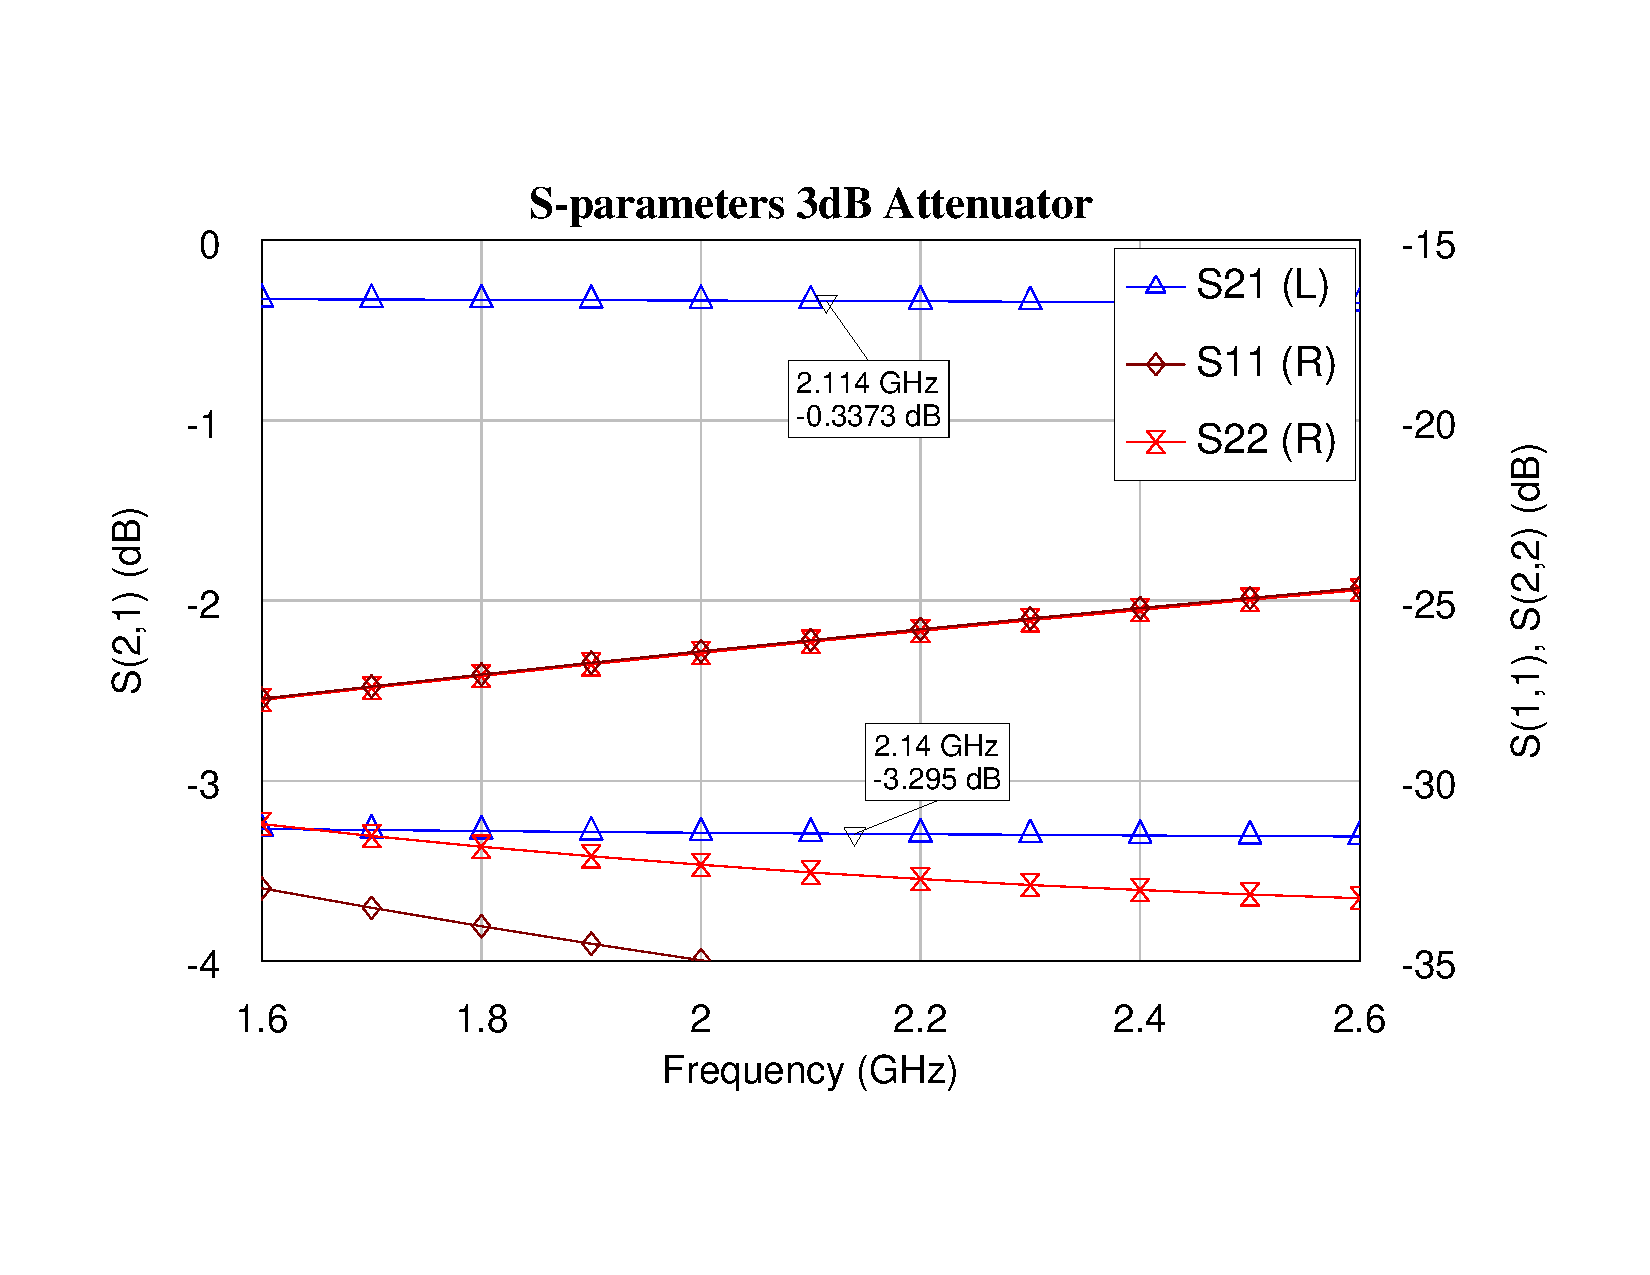
\includegraphics[width=1.0\textwidth]{fig/attenuators/S_params_3dB}
%			\caption[The S-parameters of the 3dB attenuator]{The S-parameters of the 3dB attenuator with PPH25SSW}\label{fig:S_params_3dB}
%		\end{figure}


		\begin{figure}[h!]
			\centering
			\includerect{1.0\textwidth}{fig/attenuators/All_attenuators_spread}
			\caption[Spread for all gain-states]{Spread for all gain states using PPH25SSW.}\label{fig:All_attenuators_spread}
		\end{figure}


		
		%In \autoref{fig:P1dB_Complete}, 
		

%		\begin{figure}[hbt!]
%			\centering
%			\includerect{1.0\textwidth}{fig/attenuators/P1dB_Complete}	
%			\caption[$P_{1dB}$ for entire attenuator-circuit]{Output power as a function of input power for  the complete attenuator-circuit. Shows the $P_{1dB}$-point.  All dampeners are in their inactive state, other states results in higher $P_{1db}$. Using PPH25NCF.}\label{fig:P1dB_Complete}
%		\end{figure}

		\begin{figure}[h!]
			\centering
			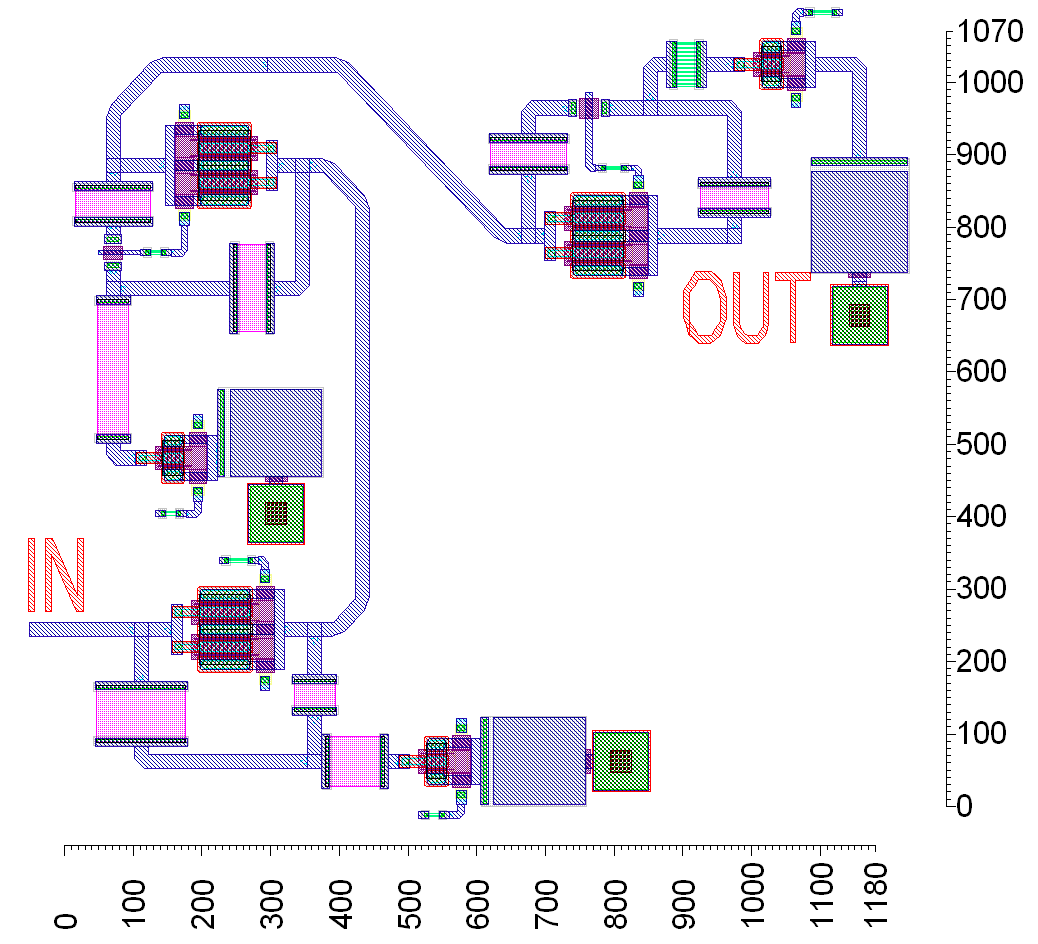
\includegraphics[width=0.8\textwidth]{fig/attenuators/attenuators_layout}
			\caption[Attenuator circuit layout]{The complete attenuator circuit.\scalemum}\label{fig:attenuators_layout}.
		\end{figure}

	
				


		
		%\begin{figure}[hbt!]
		%	\centering
		%	\includegraphics[width=1.0\textwidth]{fig/attenuators/All_attenuators}
		%	\caption{The complete attenuator circuit.}\label{fig:P1dB_Complete}
		%\end{figure}

%%%%%%%%%%%%%%%%%%%%%%%%%%%%%%%%%%%%%%%%%%%%%%%%%%%%%%%%%%%%%%%%%%%%%%%%%%%%%%%%%%%%%%%%%%%%%%%%%%%%%%%%%%%%%%%%%%%%%%%%%%%%%%%%%%
%%%%%%%%%%%%%%%%%%%%%%%%%%%%%%%%%%%%%%%%%%%%%%%%%%%%%%%%%%%%%%%%%%%%%%%%%%%%%%%%%%%%%%%%%%%%%%%%%%%%%%%%%%%%%%%%%%%%%%%%%%%%%%%%%%
\section{Attenuator control}

	\subsection{Introduction}
		The attenuators are controlled by applying either \unit[5]{V} or \unit[3]{V} to the FET's gates, thereby switching them between completely on and completely off. This is the task of the so called level shifters. The level shifters take as input a binary zero (\unit[0-.4]{V}) or one (\unit[1.8-5]{V}), adhering to the standardized LvTTL-logic.\autocite{lvttl11} % Double check these values for pph225
		
		This technique is well established at SAAB and there are existing models for the PH25-process\autocite{gustavsson07}. The level shifters are implemented again in PPH25 without any major changes.
		
	\subsection{Design}
		The schematic  and real layout for the level shifter are seen in \autoref{fig:level_shifter_sch} and \autoref{fig:level_shifter_layout}, respectively.
		In short, $v_{control}$  directly controls $T1$. When $T1$ is closed, $v_1=\unit[3]{V}$ as the bias voltage will split over $R_2$ and $R_6$. This in turn will cause $T_2$ to open, making  $v_2=\unit[5]{V}$. As $v_{control}$ is decreased, $T_1$ will eventually open, making $v_1=\unit[5]{V}$. As there will no longer be any current over $R_6$, $v_{gs}$ over $T_2$ will decrease, and $T_2$ will close, making $v_2=\unit[3]{V}$.
		
		The level shifter's output is shown in Figure\autoref{fig:levelshifter_output_spread}. By adjusting the two resistances between $V_{control}$ and ground in the circuit, the voltage at which the attenuator is turned on, $V_{shift}$ is adjusted. Also, the current consumption can be decreased by increasing the remaining resistances. However, there comes the penalty in the form of increased size. See Figure\autoref{fig:levelshifter_current} for the current consumption.


		\begin{figure}[h!]
			\centering
			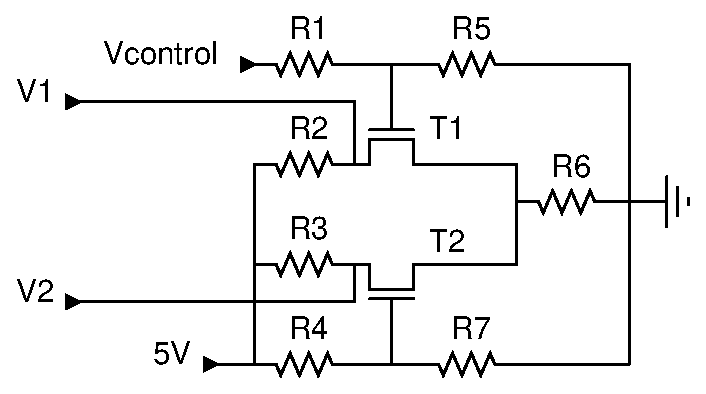
\includegraphics[width=0.7\textwidth]{fig/attenuators/sch_level_shifter}
			\caption[Level-shifter schematic layout]{Schematic of the level-shifter used for biasing the attenuators. $T_1,T_2$=\unit[1$\times$25]{\mum}, $R_1=\unit[1.0]{k\Omega}$, $R_2=\unit[2.1]{k\Omega}$, $R_3=\unit[3.3]{k\Omega}$, $R_4=\unit[20]{k\Omega}$, $R_5=\unit[6.2]{k\Omega}$, $R_6=\unit[3.0]{k\Omega}$ and $R_7=\unit[5.0]{k\Omega}$.}\label{fig:level_shifter_sch}
		\end{figure}
		
		
		\begin{figure}[h!]
			\centering
			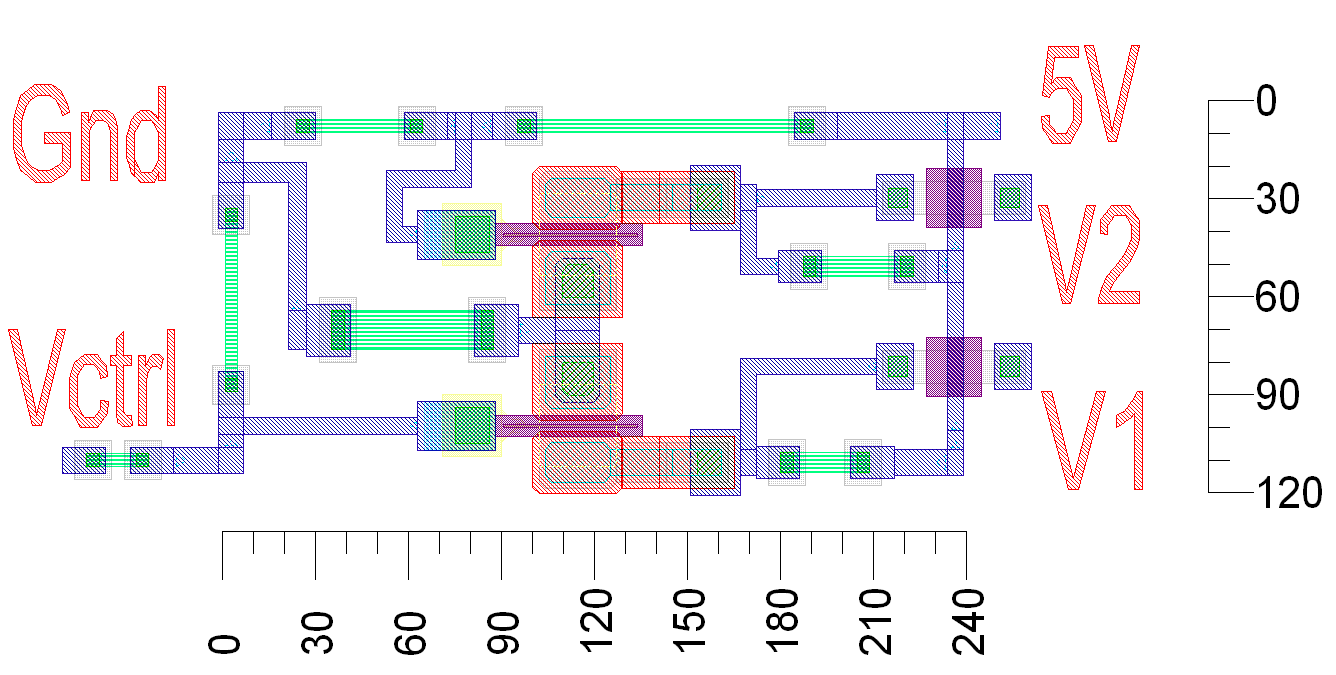
\includegraphics[width=1.0\textwidth]{fig/attenuators/level_shifter_layout}
			\caption[Level shifter layout]{The layout on-chip for the level shifter used for biasing the attenuators.}\label{fig:level_shifter_layout}
		\end{figure}


	\begin{figure}[h!]
			\centering 
			\subfloat[][Level shifter output with yield analysis.]{
				\includerect{0.5\textwidth}{fig/attenuators/level_shifter_output_spread}
				\label{fig:levelshifter_output_spread}
			}
			\subfloat[][Level shifter current consumption with yield analysis.]{
				\includerect{0.5\textwidth}{fig/attenuators/level_shifter_current}
				\label{fig:levelshifter_current}
			} 
			\caption[Level shifter output]{\subref{fig:levelshifter_output_spread} Voltages generated by the level shifter and \subref{fig:levelshifter_current} current consumption as a function of the control signal.}\label{fig:level_shifter_data}
		\end{figure}

		
%		\begin{figure}[hbt!]
%			\centering
%			\includerect{1.0\textwidth}{fig/attenuators/level_shifter_output_spread}
%			\caption[Level shifter output]{The voltages generated by the level shifter as a function of the control signal. Spread analysis is applied.}\label{fig:level_shifter_current}
%		\end{figure}
		


%		\begin{figure}[hbt!]
%			\centering
%			\includerect{1.0\textwidth}{fig/attenuators/level_shifter_current}
%			\caption[Level shifter current use]{The current consumption of the level shifter for different control signals.}\label{fig:level_shifter_current}
%		\end{figure}




